  \chapter{Evaluation}\label{ch:evaluation}


  This chapter evaluates whether \textsc{Smile} can express and execute
  schema changes consistently across the full $4 \times 4$ scenario
  matrix and whether target export preserves that consistency. To
  this end, all 16 directions are considered, which comprise 4
  intra-system evolution cases and 12 inter-system migration cases,
  and each direction is instantiated in both grammar variants.

  \section{Test Schema Design--Northwind Schema}\label{sec:test-schema}


As a common schema basis a subset of the Northwind dataset is used,
  which comprises 8~entities (e.g., \texttt{orders}, \texttt{products},
  \texttt{employees}), 69~attributes, and 8~relationships defined by
  foreign keys, where one of those references points back to its own
  table and one constitutes a composite primary key. These entities
  were selected to cover the structural patterns that are most
  relevant to migration across paradigms, such as chains of foreign
  keys that span multiple tables, nested address fields, hierarchies
  that reference themselves, and composite keys. Each paradigm has
  its own native representation of this subset, and applying both
  grammar variants across all directions yields 32~test configurations
  in total. Figures~\ref{fig:nw-pg}--\ref{fig:nw-cass} show the four
  representations native to each paradigm.

  %% =============================================================
  %% (a) PostgreSQL ER ===========================================
  %% =============================================================
\begin{figure}[htbp]
\centering
\resizebox{\textwidth}{!}{%
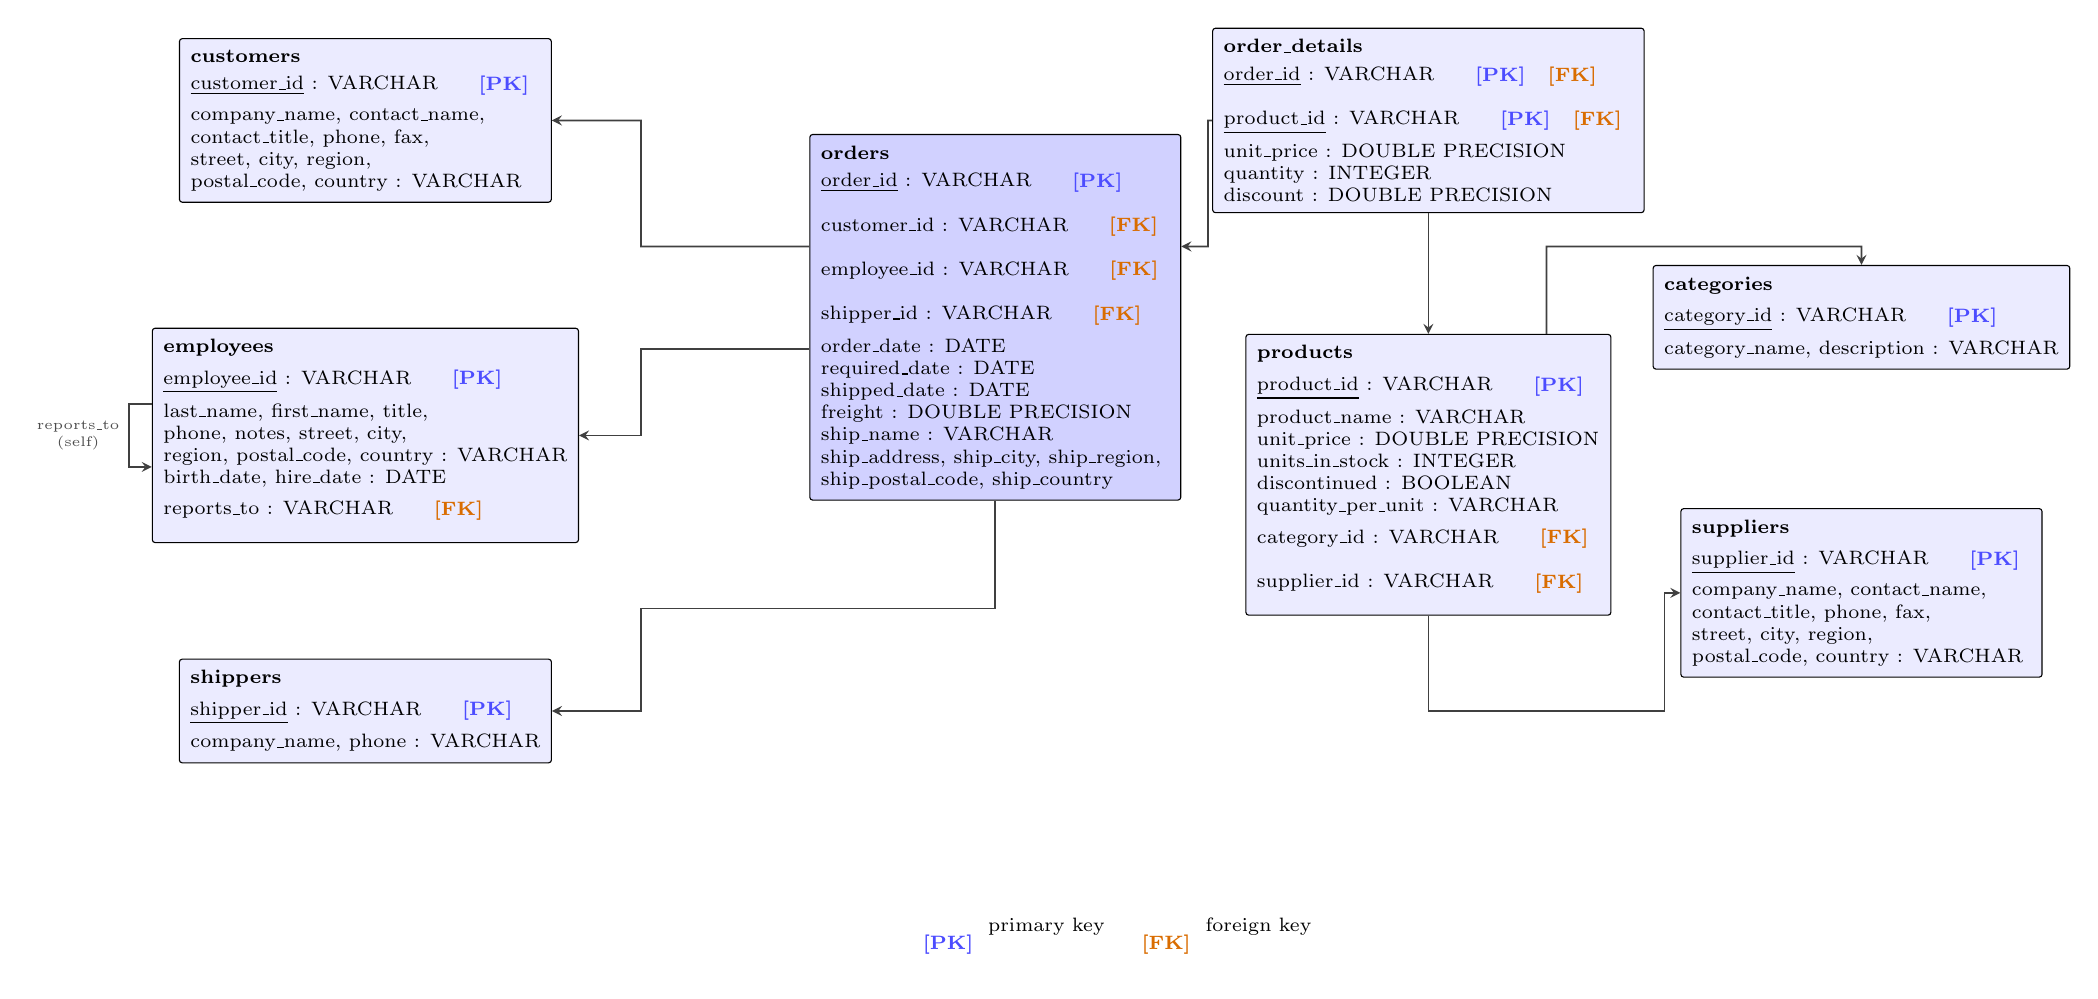
\begin{tikzpicture}[
  font=\scriptsize,
  tbl/.style={draw, rectangle, rounded corners=1pt, align=left,
              inner sep=4pt, fill=blue!8},
  pkt/.style={tbl, fill=blue!18},
  arr/.style={->, >=stealth, semithick, black!75},
  pktag/.style={font=\scriptsize\bfseries, text=blue!70},
  fktag/.style={font=\scriptsize\bfseries, text=orange!85!black}
]
  \node[pkt] (ord) at (5.5, 0) {%
    \textbf{orders}\\
    \underline{order\_id} : VARCHAR \quad\tikz[baseline=-0.5ex]{\node[pktag]{[PK]};}\\
    customer\_id : VARCHAR \quad\tikz[baseline=-0.5ex]{\node[fktag]{[FK]};}\\
    employee\_id : VARCHAR \quad\tikz[baseline=-0.5ex]{\node[fktag]{[FK]};}\\
    shipper\_id : VARCHAR \quad\tikz[baseline=-0.5ex]{\node[fktag]{[FK]};}\\
    order\_date : DATE\\
    required\_date : DATE\\
    shipped\_date : DATE\\
    freight : DOUBLE PRECISION\\
    ship\_name : VARCHAR\\
    ship\_address, ship\_city, ship\_region,\\
    ship\_postal\_code, ship\_country};
  \node[tbl] (cu) at (-2.5, 2.5) {%
    \textbf{customers}\\
    \underline{customer\_id} : VARCHAR \quad\tikz[baseline=-0.5ex]{\node[pktag]{[PK]};}\\
    company\_name, contact\_name,\\
    contact\_title, phone, fax,\\
    street, city, region,\\
    postal\_code, country : VARCHAR};
  \node[tbl] (em) at (-2.5, -1.5) {%
    \textbf{employees}\\
    \underline{employee\_id} : VARCHAR \quad\tikz[baseline=-0.5ex]{\node[pktag]{[PK]};}\\
    last\_name, first\_name, title,\\
    phone, notes, street, city,\\
    region, postal\_code, country : VARCHAR\\
    birth\_date, hire\_date : DATE\\
    reports\_to : VARCHAR \quad\tikz[baseline=-0.5ex]{\node[fktag]{[FK]};}};
  \node[tbl] (sh) at (-2.5, -5.0) {%
    \textbf{shippers}\\
    \underline{shipper\_id} : VARCHAR \quad\tikz[baseline=-0.5ex]{\node[pktag]{[PK]};}\\
    company\_name, phone : VARCHAR};
  \node[tbl] (od) at (11, 2.5) {%
    \textbf{order\_details}\\
    \underline{order\_id} : VARCHAR \quad\tikz[baseline=-0.5ex]{\node[pktag]{[PK]};}\tikz[baseline=-0.5ex]{\node[fktag]{[FK]};}\\
    \underline{product\_id} : VARCHAR \quad\tikz[baseline=-0.5ex]{\node[pktag]{[PK]};}\tikz[baseline=-0.5ex]{\node[fktag]{[FK]};}\\
    unit\_price : DOUBLE PRECISION\\
    quantity : INTEGER\\
    discount : DOUBLE PRECISION};
  \node[tbl] (pr) at (11, -2.0) {%
    \textbf{products}\\
    \underline{product\_id} : VARCHAR \quad\tikz[baseline=-0.5ex]{\node[pktag]{[PK]};}\\
    product\_name : VARCHAR\\
    unit\_price : DOUBLE PRECISION\\
    units\_in\_stock : INTEGER\\
    discontinued : BOOLEAN\\
    quantity\_per\_unit : VARCHAR\\
    category\_id : VARCHAR \quad\tikz[baseline=-0.5ex]{\node[fktag]{[FK]};}\\
    supplier\_id : VARCHAR \quad\tikz[baseline=-0.5ex]{\node[fktag]{[FK]};}};
  \node[tbl] (ca) at (16.5, 0) {%
    \textbf{categories}\\
    \underline{category\_id} : VARCHAR \quad\tikz[baseline=-0.5ex]{\node[pktag]{[PK]};}\\
    category\_name, description : VARCHAR};
  \node[tbl] (su) at (16.5, -3.5) {%
    \textbf{suppliers}\\
    \underline{supplier\_id} : VARCHAR \quad\tikz[baseline=-0.5ex]{\node[pktag]{[PK]};}\\
    company\_name, contact\_name,\\
    contact\_title, phone, fax,\\
    street, city, region,\\
    postal\_code, country : VARCHAR};

  %% orders -> customers  (FK: orders.customer_id -> customers.customer_id)
  \draw[arr] ([yshift=0.9cm]ord.west) -- (1.0, 0.9) -- (1.0, 2.5) -- (cu.east);

  %% orders -> employees  (FK: orders.employee_id -> employees.employee_id)
  \draw[arr] ([yshift=-0.4cm]ord.west) -- (1.0, -0.4) -- (1.0, -1.5) -- (em.east);

  %% orders -> shippers   (FK: orders.shipper_id  -> shippers.shipper_id)
  \draw[arr] (ord.south) -- (5.5, -3.7) -- (1.0, -3.7) -- (1.0, -5.0) -- (sh.east);

  %% order_details -> orders (east-upper)
  \draw[arr] (od.west) -- (8.2, 2.5) -- (8.2, 0.9) -- ([yshift=0.9cm]ord.east);

  %% order_details -> products (vertical)
  \draw[arr] (od.south) -- (pr.north);

  %% products -> categories (enter via north)
  \draw[arr] ([xshift=1.5cm]pr.north) -- (12.5, 0.9) -- (16.5, 0.9) -- (ca.north);

  %% products -> suppliers (exit south, route under)
  \draw[arr] (pr.south) -- (11, -5.0) -- (14.0, -5.0) -- (14.0, -3.5) -- (su.west);

  %% reports_to self-loop on left of employees
  \draw[arr] ([yshift=0.4cm]em.west) -- (-5.5, -1.1) -- (-5.5, -1.9) -- ([yshift=-0.4cm]em.west);
  \node[font=\tiny, anchor=east, text=black!70, align=center]
    at (-5.5, -1.5) {reports\_to\\(self)};

  \node[font=\scriptsize, anchor=north]
    at (7, -7.5) {%
    \tikz[baseline=-0.5ex]{\node[pktag]{[PK]};} primary key \quad
    \tikz[baseline=-0.5ex]{\node[fktag]{[FK]};} foreign key};
\end{tikzpicture}}
\caption{Northwind subset in PostgreSQL SQL.}
\label{fig:nw-pg}
\end{figure}

  %% =============================================================
  %% (b) MongoDB JSON Schema (compact, fits one page) ===========
  %% =============================================================
  \begin{figure}[htbp]
  \centering
  \begin{minipage}{0.95\textwidth}
  \begin{lstlisting}[basicstyle=\ttfamily\scriptsize,
                     backgroundcolor=\color{green!4},
                     frame=single, framesep=3pt,
                     xleftmargin=4pt, basewidth=0.5em,
                     keepspaces=true]
{ "collections": {
    "orders": {                                  // root collection #1
      "_id": string,                             // unique identifier
      "customer_id": string,                     // cross-coll ref -> customers._id, required
      "order_date", "required_date", "shipped_date": date,
      "freight": double, "ship_name": string,
      "ship_destination": {                      // L1, required
        "ship_address", "ship_city", "ship_region",
        "ship_postal_code", "ship_country": string },
      "employee": {                              // L1, required
        "last_name", "first_name", "title": string,
        "birth_date", "hire_date": date,
        "phone", "notes", "reports_to": string,
        "address": {                             // L2, required
          "street", "city", "region", "postal_code", "country": string }},
      "shipper": { "company_name", "phone": string },          // L1, required
      "details": [ {                             // L1, array, required
        "unit_price": double, "quantity": int, "discount": double,
        "product": {                             // L2, required
          "product_name", "quantity_per_unit": string,
          "unit_price": double, "units_in_stock": int, "discontinued": bool,
          "category":  { "category_name", "description": string },        // L3, required
          "supplier":  {                                                  // L3, required
            "company_name", "contact_name", "contact_title",
            "phone", "fax", "street", "city", "region",
            "postal_code", "country": string }}}]
    },
    "customers": {                               // root collection #2
      "_id": string,                             // unique identifier
      "company_name", "contact_name", "contact_title",
      "phone", "fax": string,
      "address": {                               // L1, required
        "street", "city", "region", "postal_code", "country": string }
    }
}}
  \end{lstlisting}
  \end{minipage}
  \caption{Northwind subset in MongoDB JSON Schema.}
  \label{fig:nw-mongo}
  \end{figure}

  %% =============================================================
  %% (c) Neo4j graph ============================================
  %% =============================================================
\begin{figure}[htbp]
\centering
\resizebox{\textwidth}{!}{%
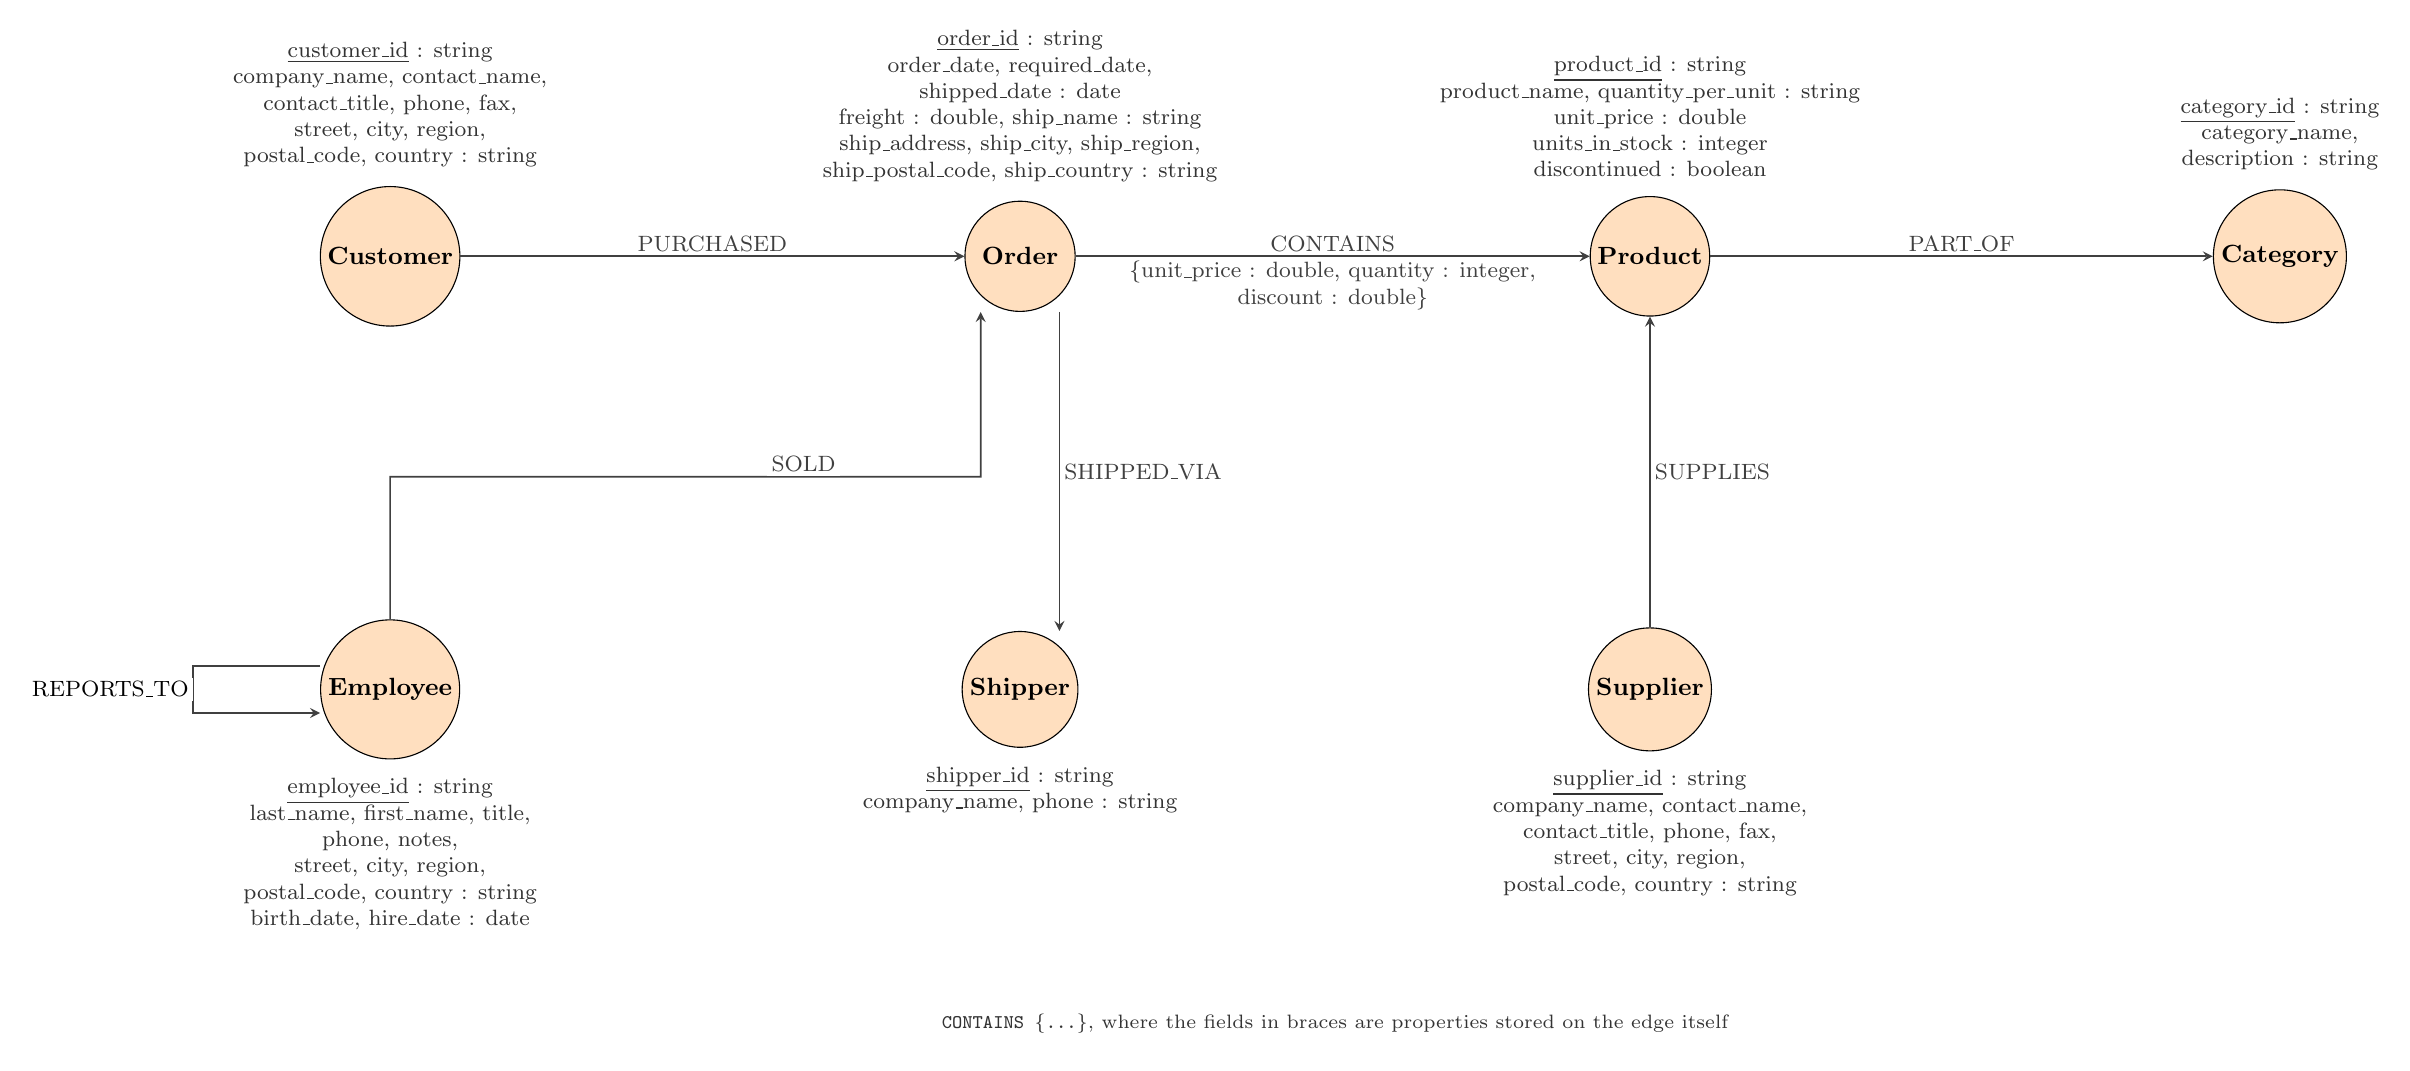
\begin{tikzpicture}[
  font=\scriptsize,
  nd/.style={draw, circle, fill=orange!25, align=center,
             inner sep=2pt, minimum size=1.4cm, font=\small\bfseries},
  prop/.style={font=\footnotesize, align=center, inner sep=1pt, text=black!80},
  arr/.style={->, >=stealth, semithick, black!75},
  edglab/.style={font=\footnotesize, fill=white, inner sep=1.5pt}
]
  %% --- Vertices : two rows aligned vertically (wider spacing) ---
  \node[nd] (cu) at (0,    2) {Customer};
  \node[nd] (or) at (8,    2) {Order};
  \node[nd] (pr) at (16,   2) {Product};
  \node[nd] (ca) at (24,   2) {Category};
  \node[nd] (em) at (0,   -3.5) {Employee};
  \node[nd] (sh) at (8,   -3.5) {Shipper};
  \node[nd] (su) at (16,  -3.5) {Supplier};
  %% --- Property lists ---
  \node[prop, anchor=south] at ([yshift=0.2cm]cu.north) {%
    \underline{customer\_id} : string\\
    company\_name, contact\_name,\\
    contact\_title, phone, fax,\\
    street, city, region,\\
    postal\_code, country : string};
  \node[prop, anchor=south] at ([yshift=0.2cm]or.north) {%
    \underline{order\_id} : string\\
    order\_date, required\_date,\\
    shipped\_date : date\\
    freight : double, ship\_name : string\\
    ship\_address, ship\_city, ship\_region,\\
    ship\_postal\_code, ship\_country : string};
  \node[prop, anchor=south] at ([yshift=0.2cm]pr.north) {%
    \underline{product\_id} : string\\
    product\_name, quantity\_per\_unit : string\\
    unit\_price : double\\
    units\_in\_stock : integer\\
    discontinued : boolean};
  \node[prop, anchor=south] at ([yshift=0.2cm]ca.north) {%
    \underline{category\_id} : string\\
    category\_name,\\
    description : string};
  \node[prop, anchor=north] at ([yshift=-0.2cm]em.south) {%
    \underline{employee\_id} : string\\
    last\_name, first\_name, title,\\
    phone, notes,\\
    street, city, region,\\
    postal\_code, country : string\\
    birth\_date, hire\_date : date};
  \node[prop, anchor=north] at ([yshift=-0.2cm]sh.south) {%
    \underline{shipper\_id} : string\\
    company\_name, phone : string};
  \node[prop, anchor=north] at ([yshift=-0.2cm]su.south) {%
    \underline{supplier\_id} : string\\
    company\_name, contact\_name,\\
    contact\_title, phone, fax,\\
    street, city, region,\\
    postal\_code, country : string};
  %% --- Relationships ---
  \draw[arr] (cu.east) -- node[edglab, above] {PURCHASED} (or.west);
  \draw[arr] (or.east) -- node[edglab, above] {CONTAINS}
                                node[edglab, below, align=center] {\{unit\_price : double, quantity : integer,\\ discount : double\}} (pr.west);
  \draw[arr] (pr.east) -- node[edglab, above] {PART\_OF} (ca.west);
  \draw[arr] (em.north) -- (0, -0.8) -- node[edglab, above, pos=0.7] {SOLD} (7.5, -0.8) -- ([xshift=-0.5cm]or.south);
  \draw[arr] ([xshift=0.5cm]or.south) -- node[edglab, right] {SHIPPED\_VIA} ([xshift=0.5cm]sh.north);
  \draw[arr] (su.north) -- node[edglab, right] {SUPPLIES} (pr.south);
  \draw[arr] ([yshift=0.3cm]em.west) -- (-2.5, -3.2) -- (-2.5, -3.8) -- ([yshift=-0.3cm]em.west);
  \node[edglab, anchor=east] at (-2.5, -3.5) {REPORTS\_TO};
  \node[font=\scriptsize, black!80, anchor=north] at (12, -7.5) {%
    \texttt{CONTAINS \{\dots\}}, where the fields in braces are properties stored on the edge itself};
\end{tikzpicture}}
\caption{Northwind subset in Neo4j Cypher.}
\label{fig:nw-neo}
\end{figure}

  %% =============================================================
  %% (d) Cassandra Chebotko (2-column to fit one page) =========
  %% =============================================================
  \begin{figure}[htbp]
  \centering
  \resizebox{\textwidth}{!}{%
  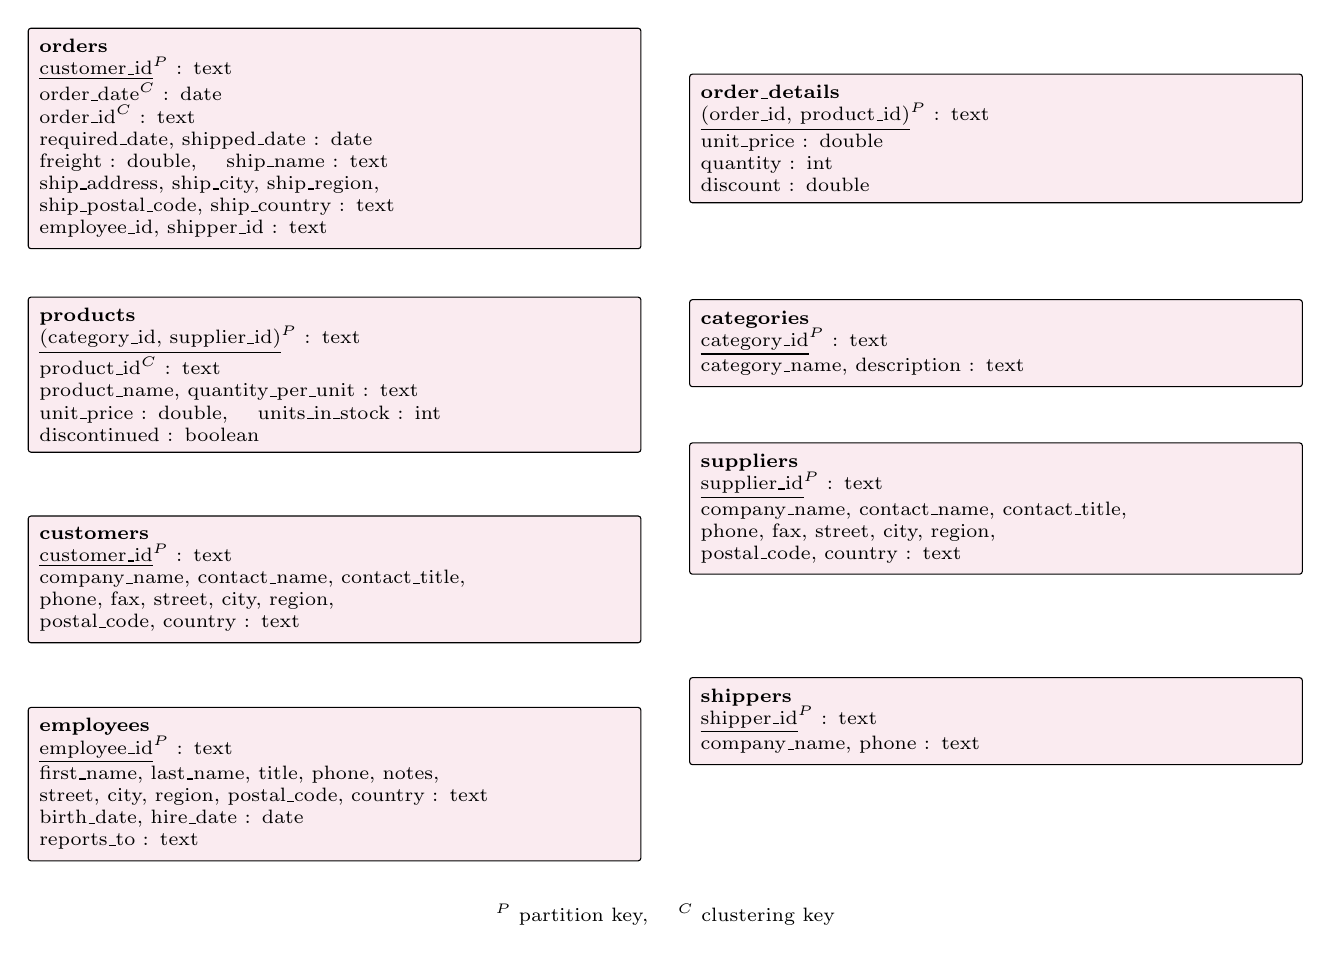
\begin{tikzpicture}[
    font=\scriptsize,
    cf/.style={draw, rectangle, rounded corners=1pt, align=left,
               inner sep=4pt, fill=purple!8, text width=7.5cm}
  ]
    %% --- Left column ---
    \node[cf] at (-4.2, 0) {%
      \textbf{orders}\\
      \underline{customer\_id}$^P$ : text\\
      order\_date$^C$ : date\\
      order\_id$^C$ : text\\
      required\_date, shipped\_date : date\\
      freight : double, \quad ship\_name : text\\
      ship\_address, ship\_city, ship\_region,\\
      ship\_postal\_code, ship\_country : text\\
      employee\_id, shipper\_id : text};
    \node[cf] at (-4.2, -3.0) {%
      \textbf{products}\\
      \underline{(category\_id, supplier\_id)}$^P$ : text\\
      product\_id$^C$ : text\\
      product\_name, quantity\_per\_unit : text\\
      unit\_price : double, \quad
      units\_in\_stock : int\\
      discontinued : boolean};
    \node[cf] at (-4.2, -5.6) {%
      \textbf{customers}\\
      \underline{customer\_id}$^P$ : text\\
      company\_name, contact\_name, contact\_title,\\
      phone, fax, street, city, region,\\
      postal\_code, country : text};
    \node[cf] at (-4.2, -8.2) {%
      \textbf{employees}\\
      \underline{employee\_id}$^P$ : text\\
      first\_name, last\_name, title, phone, notes,\\
      street, city, region, postal\_code, country : text\\
      birth\_date, hire\_date : date\\
      reports\_to : text};

    %% --- Right column ---
    \node[cf] at (4.2, 0) {%
      \textbf{order\_details}\\
      \underline{(order\_id, product\_id)}$^P$ : text\\
      unit\_price : double\\
      quantity : int\\
      discount : double};
    \node[cf] at (4.2, -2.6) {%
      \textbf{categories}\\
      \underline{category\_id}$^P$ : text\\
      category\_name, description : text};
    \node[cf] at (4.2, -4.7) {%
      \textbf{suppliers}\\
      \underline{supplier\_id}$^P$ : text\\
      company\_name, contact\_name, contact\_title,\\
      phone, fax, street, city, region,\\
      postal\_code, country : text};
    \node[cf] at (4.2, -7.4) {%
      \textbf{shippers}\\
      \underline{shipper\_id}$^P$ : text\\
      company\_name, phone : text};

    \node[font=\scriptsize, anchor=north]
      at (0, -9.6) {$^P$~partition key, \quad $^C$~clustering key};
  \end{tikzpicture}}
  \caption{Northwind subset in Cassandra CQL.}
  \label{fig:nw-cass}
  \end{figure}

  After reverse engineering, each adapter produces a paradigm-specific
  Meta~V1 in M-Model$^{+}$ (Figure~\ref{fig:nw-meta-v1}). The four
  representations share the same vocabulary
  (\textit{EntityType}, \textit{Property}, \textit{Reference},
  \textit{Embedded}, \textit{Edge}), but their topologies differ
  because each adapter assigns a different \texttt{EntityKind} per
  entity. PostgreSQL produces 8~\texttt{TABLE} entities connected by
  FK \textit{Reference} edges; MongoDB produces 2~\texttt{DOCUMENT}
  roots with \texttt{EMBEDDED} sub-entities forming containment trees;
  Neo4j produces 7~\texttt{VERTEX} entities and 7~\texttt{EDGE}
  entities (one carrying edge properties); Cassandra produces
  8~\texttt{WIDE\_COLUMN\_TABLE} entities with no enforced
  \textit{References} (FK columns survive as plain \texttt{TEXT}).
  \textsc{Smile} operators and the Layer~1 normalizer reconcile these
  shapes during transformation and validation.

  %% =============================================================
  %% (e) Meta V1 as one JSON file with divergences highlighted ====
  %% Black text = shared across all 4 adapters
  %% Coloured boxes = paradigm-specific values
  %%   blue   = PostgreSQL   green  = MongoDB
  %%   orange = Neo4j        purple = Cassandra
  %% =============================================================
\begin{figure}[htbp]
\centering
\providecommand{\BPG}[1]{{\setlength{\fboxsep}{1pt}\colorbox{blue!22}{\vphantom{Mg}#1}}}
\providecommand{\BMg}[1]{{\setlength{\fboxsep}{1pt}\colorbox{green!28}{\vphantom{Mg}#1}}}
\providecommand{\BNe}[1]{{\setlength{\fboxsep}{1pt}\colorbox{orange!35}{\vphantom{Mg}#1}}}
\providecommand{\BCs}[1]{{\setlength{\fboxsep}{1pt}\colorbox{purple!22}{\vphantom{Mg}#1}}}
\begin{lstlisting}[basicstyle=\ttfamily\tiny,
                   backgroundcolor=\color{gray!4},
                   frame=single, framesep=6pt,
                   xleftmargin=6pt, basewidth=0.5em,
                   keepspaces=true,
                   escapeinside={(*}{*)}]
{
  "db_name": "northwind",  "version": 1,                                     /* shared */

  /* ============= DIVERGENCE 1 / 4: db_type ============= */
  "db_type":  (*\BPG{"relational"}*) | (*\BMg{"document"}*) | (*\BNe{"graph"}*) | (*\BCs{"columnar"}*),

  "entity_types": {

    "orders": {
      (*{\color{red}\bfseries\vphantom{Mg}[Note: the \texttt{orders} entity is shown here in full as a worked example;}*)
      (*{\color{red}\bfseries\vphantom{Mg} the other 7 entities appear in one-line summary form further below.]}*)

      /* ----- shared entity-level metadata ----- */
      "meta_id":     "E:orders",
      "object_name": ["orders"],
      "is_root":     true,
      "constraints": [
        { "constraint_type":   "unique",
          "unique_properties": [
            { "primary_key_type": "simple",
              "property_id":      "P:orders:order_id" }
          ]
        }
      ],

      /* ============= DIVERGENCE 2 / 4: orders.entity_kind ============= */
      "entity_kind": (*\BPG{"table"}*) | (*\BMg{"document"}*) | (*\BNe{"vertex"}*) | (*\BCs{"wide\_column\_table"}*),

      "properties": [
        /* one full exemplar showing all 6 fields produced by Property.to_dict(): */
        { "kind":"property", "meta_id":"P:orders:order_id", "name":"order_id",
          "data_type":{"kind":"primitive","type":"string"}, "is_key":true, "is_optional":false },

        /* the remaining 10 share the same shape; abbreviated as {name, type} pairs */
        {name:"order_date","date"},      {name:"required_date","date"},   {name:"shipped_date","date"},
        {name:"freight","double"},       {name:"ship_name","string"},
        {name:"ship_address","string"},  {name:"ship_city","string"},     {name:"ship_region","string"},
        {name:"ship_postal_code","string"}, {name:"ship_country","string"},

        /* ============= DIVERGENCE 3 / 4: which adapters keep the 3 FK columns as plain string properties ============= */
        (*\BPG{[PG]}\BCs{[Cs]}*):  ,  {name:"customer_id"}, {name:"employee_id"}, {name:"shipper_id"}
        (*\BMg{[Mg]}*):            ,  {name:"customer_id"}     // only this one (cross-coll ref to customers root)
        (*\BNe{[Ne]}*):               (none kept -- all 3 replaced by EDGE entities below)
      ],

      /* ============= DIVERGENCE 4 / 4: orders.relationships ============= */
      "relationships":
         (*\BPG{[ \{kind:"reference", refs\_to:"customers"\},}*)
         (*\BPG{  \{kind:"reference", refs\_to:"employees"\},}*)
         (*\BPG{  \{kind:"reference", refs\_to:"shippers"\}  ]}*)
         (*\BMg{[ \{kind:"reference", refs\_to:"customers"\} (cross-collection),}*)
         (*\BMg{  \{kind:"embedded",  aggregates:"employee"\},}*)
         (*\BMg{  \{kind:"embedded",  aggregates:"shipper"\},}*)
         (*\BMg{  \{kind:"embedded",  aggregates:"ship\_destination"\},}*)
         (*\BMg{  \{kind:"embedded",  aggregates:"details"\}  ]}*)
         (*\BNe{[ ]    // graph: relationships are top-level EDGE entities (see below)}*)
         (*\BCs{[ ]    // columnar: CQL has no FOREIGN KEY syntax; FK columns above are plain string properties}*)
    },

    /* ============= the 7 other entities: same shared shape (meta_id, object_name, is_root, constraints, properties, relationships); */
    /*                                     entity_kind diverges by paradigm, plus per-entity property/relationship summary             */
    "order_details": { entity_kind: (*\BPG{"table"}*)|(*\BMg{"embedded"}*)|(*\BNe{"edge"}*)|(*\BCs{"wide\_column\_table"}*),
                       5 props (composite PK [order_id, product_id] + 1 int + 2 doubles),
                       2 outgoing References [relational only]; document flattens via Embedded array;
                       graph IS the CONTAINS edge; columnar has no References },
    "customers":     { entity_kind: (*\BPG{"table"}*)|(*\BMg{"document"}*)|(*\BNe{"vertex"}*)|(*\BCs{"wide\_column\_table"}*),
                       11 props (1 PK + 10 string),
                       0 outgoing relationships (target of orders.customer_id Reference) },
    "employees":     { entity_kind: (*\BPG{"table"}*)|(*\BMg{"embedded"}*)|(*\BNe{"vertex"}*)|(*\BCs{"wide\_column\_table"}*),
                       14 props (1 PK + 10 string + 2 date + 1 self-FK reports_to),
                       1 self-Reference [relational + columnar only];
                       document embeds employee under orders; graph uses REPORTS_TO edge },
    "shippers":      { entity_kind: (*\BPG{"table"}*)|(*\BMg{"embedded"}*)|(*\BNe{"vertex"}*)|(*\BCs{"wide\_column\_table"}*),
                       3 props (1 PK + 2 string),
                       0 outgoing relationships (target of orders.shipper_id Reference) },
    "products":      { entity_kind: (*\BPG{"table"}*)|(*\BMg{"embedded"}*)|(*\BNe{"vertex"}*)|(*\BCs{"wide\_column\_table"}*),
                       8 props (1 PK + 1 string + 1 double + 1 int + 1 bool + 1 string
                                + 2 FK columns supplier_id/category_id),
                       2 outgoing References [relational only];
                       document embeds; graph uses SUPPLIES + PART_OF edges; columnar has no References },
    "categories":    { entity_kind: (*\BPG{"table"}*)|(*\BMg{"embedded"}*)|(*\BNe{"vertex"}*)|(*\BCs{"wide\_column\_table"}*),
                       3 props (1 PK + 2 string),
                       0 outgoing relationships (target of products.category_id Reference) },
    "suppliers":     { entity_kind: (*\BPG{"table"}*)|(*\BMg{"embedded"}*)|(*\BNe{"vertex"}*)|(*\BCs{"wide\_column\_table"}*),
                       11 props (1 PK + 10 string),
                       0 outgoing relationships (target of products.supplier_id Reference) }

    /* ============= graph paradigm only: ALL 7 EDGE entities (peer to the 7 VERTEX entities above) ============= */
    /* PURCHASED/SOLD/SHIPPED_VIA replace the 3 relational References on orders.                            */
    /* CONTAINS replaces the order_details join table and uniquely carries edge.properties.             */
    /* PART_OF/SUPPLIES replace the 2 References on products. REPORTS_TO replaces employees.reports_to. */
    (*\BNe{, "PURCHASED"    : \{kind:"edge", source: customers --> orders,    card: 0..n\}}*)
    (*\BNe{  "SOLD"         : \{kind:"edge", source: employees --> orders,    card: 0..n\}}*)
    (*\BNe{  "SHIPPED\_VIA"  : \{kind:"edge", source: orders    --> shippers,  card: 0..n\}}*)
    (*\BNe{  "CONTAINS"     : \{kind:"edge", source: orders    --> products,  card: 0..n,}*)
    (*\BNe{                    edge.properties=[unit\_price:double, quantity:integer, discount:double]\}}*)
    (*\BNe{  "PART\_OF"      : \{kind:"edge", source: products  --> categories,card: 0..n\}}*)
    (*\BNe{  "SUPPLIES"     : \{kind:"edge", source: suppliers --> products,  card: 0..n\}}*)
    (*\BNe{  "REPORTS\_TO"   : \{kind:"edge", source: employees --> employees, card: 0..n\}    // self-loop}*)
  }
}
\end{lstlisting}

\smallskip
{\footnotesize DB schemas:\quad
\BPG{~relational~}\quad
\BMg{~document~}\quad
\BNe{~graph~}\quad
\BCs{~columnar~}}

\caption{Meta V1 in M-Model$^{+}$ JSON form.}
\label{fig:nw-meta-v1}
\end{figure}

\section{Migration Scenarios}\label{sec:eval-migration}

Each of the 12 off-diagonal directions in the 4$\times$4 matrix takes a Northwind schema in one paradigm and rewrites it in another, keeping the same business content. \Cref{fig:nw-meta-v2-migration} lists the operation chain for every direction, and across all 12 the chains look almost the same. Most of every script is routine \texttt{ADD}, \texttt{DELETE}, and \texttt{RENAME} operations on properties, entities, and embeddings, recurring in nearly identical form whichever two paradigms are being bridged. \textsc{Smile} is built on a single meta model shared by all four paradigms, so an operation that edits the meta model behaves the same way no matter which paradigm is involved. The handful of operations that need to differ all sit at the few structural points where the paradigms diverge.

There are five of them. \texttt{NEST} and \texttt{UNNEST} sit at the document boundary on the many side, where a child entity becomes an embedded array. This happens six times in every direction into MongoDB and six times in every direction out of it. \texttt{FLATTEN} and \texttt{UNFLATTEN} do the same job on the one side of the same boundary, folding an embedded object's fields into its parent or grouping them back out, three times each direction. \texttt{TRANSFORM} handles the trickier case at the graph boundary, where a junction table already carries its own properties. On the way in, it lifts the table into an edge with edge properties. On the way out, it pushes the edge back into a separate entity. Simple foreign keys without their own properties take a shorter path, so that \texttt{DELETE\_FOREIGN\_KEY} drops the constraint, \texttt{ADD\_ENTITY} introduces the edge, and the inverse pair restores them in the reverse direction. Foreign keys are created or deleted at the relational boundary, since they are a relational concept. Cassandra is
  unusual in having the schema itself decide how rows sit on the cluster, where each table has a partition key that picks which node a row goes to and a clustering key
  that fixes the order of rows within that node.


Across the 12 scripts the same five concerns recur on top of a shared core of \texttt{ADD}, \texttt{DELETE}, and \texttt{RENAME} operations. Three principles shaped
  how the scripts were written. Every operation earns its place by bridging an actual gap between two paradigms, keeping the script minimal. The scripts also work
  entirely within the schema, dealing with structural elements such as entities, properties, keys, references, and embeddings, while instance data, queries, and
  application code stay on the data side. Each paradigm-specific operation comes with an inverse. \texttt{UNNEST} undoes \texttt{NEST}, \texttt{UNFLATTEN} undoes          \texttt{FLATTEN}, \texttt{DELETE\_FOREIGN\_KEY} undoes \texttt{ADD\_FOREIGN\_KEY}, \texttt{DELETE\_PARTITION\_KEY} undoes \texttt{ADD\_PARTITION\_KEY}, and
  \texttt{DELETE\_CLUSTERING\_KEY} undoes \texttt{ADD\_CLUSTERING\_KEY}. \texttt{TRANSFORM} is itself bidirectional, switching between \texttt{INTO RELATIONSHIP} and
  \texttt{INTO ENTITY} according to direction. The round trip $A \to B \to A$ is therefore the forward script applied operation by operation in reverse.


\begin{figure}[htbp]
\centering
\footnotesize
\begin{tabularx}{\textwidth}{@{}p{3.5cm} X@{}}
\toprule
\textbf{Direction} & \textbf{Migration test script summary} \\
\midrule

relational $\to$ document
 & \texttt{NEST} $\times$6 (aggregate child entities into the two document trees orders + customers);
   \texttt{UNFLATTEN} $\times$3 (group flat address columns into nested sub-objects);
   \texttt{DELETE\_ENTITY} $\times$6 (drop entities now embedded inside their parent);
   \texttt{DELETE\_FK} $\times$1 (customer\_id stays as cross-collection reference) \\
\midrule

relational $\to$ graph
 & \texttt{TRANSFORM} order\_details $\to$ \texttt{CONTAINS} edge (collapse the join table into an edge that carries edge properties);
   \texttt{DELETE\_FK} $\times$8 (graph has no FK enforcement; relations live as \texttt{EDGE} entities) \\
\midrule

relational $\to$ columnar
 & \texttt{DELETE\_FK} $\times$8 (CQL has no \texttt{FOREIGN KEY} syntax);
   \texttt{ADD\_PARTITION\_KEY} $\times$3 (assign partition keys for query-driven access);
   \texttt{ADD\_CLUSTERING\_KEY} $\times$3 (preserve sort order inside the partition) \\
\midrule

document $\to$ relational
 & \texttt{UNNEST} $\times$6 (extract embedded sub-documents into top-level tables);
   \texttt{FLATTEN} $\times$3 (lift address sub-objects to flat columns);
   \texttt{ADD\_PK} $\times$6 (each new top-level entity needs a primary key);
   \texttt{ADD\_FK} $\times$8 (recover FK enforcement that documents avoid by embedding) \\
\midrule

document $\to$ graph
 & \texttt{UNNEST} $\times$6 (extract sub-documents into graph vertices);
   \texttt{FLATTEN} $\times$3 (lift address fields);
   \texttt{ADD\_PK} $\times$6 (vertices need a node key);
   \texttt{TRANSFORM} order\_details $\to$ \texttt{CONTAINS} (convert join data into an edge with edge properties) \\
\midrule

document $\to$ columnar
 & \texttt{UNNEST} $\times$6 (extract sub-documents into wide-column tables);
   \texttt{FLATTEN} $\times$3 (lift address fields);
   \texttt{ADD\_PK} $\times$5 (most new tables need a simple PK before re-keying);
   \texttt{ADD\_PARTITION\_KEY} $\times$3 + \texttt{ADD\_CLUSTERING\_KEY} $\times$3 (Cassandra-style query-driven access keys) \\
\midrule

graph $\to$ relational
 & \texttt{TRANSFORM} \texttt{CONTAINS} $\to$ \texttt{ENTITY} (materialise the edge as the join table order\_details);
   \texttt{DELETE\_ENTITY} $\times$6 (remove the remaining \texttt{EDGE} entities);
   \texttt{ADD\_PK} $\times$1 (composite PK for the new join table);
   \texttt{ADD\_FK} $\times$8 (recover FK enforcement that the graph paradigm omits) \\
\midrule

graph $\to$ document
 & \texttt{TRANSFORM} \texttt{CONTAINS} $\to$ \texttt{ENTITY} (materialise the edge as a regular entity first);
   \texttt{NEST} $\times$6 (aggregate the entities into document trees);
   \texttt{UNFLATTEN} $\times$3 (group address fields);
   \texttt{DELETE\_ENTITY} $\times$12 (remove the 7 \texttt{EDGE} entities + the 5 entities now embedded) \\
\midrule

graph $\to$ columnar
 & \texttt{TRANSFORM} \texttt{CONTAINS} $\to$ \texttt{ENTITY} (edge $\to$ table);
   \texttt{DELETE\_ENTITY} $\times$6 (remove remaining \texttt{EDGE} entities);
   \texttt{ADD\_PARTITION\_KEY} $\times$3 + \texttt{ADD\_CLUSTERING\_KEY} $\times$3 (Cassandra access keys) \\
\midrule

columnar $\to$ relational
 & \texttt{DELETE\_PARTITION\_KEY} $\times$3 + \texttt{DELETE\_CLUSTERING\_KEY} $\times$3 (drop Cassandra-specific keys);
   \texttt{ADD\_PK} $\times$3 (re-establish simple primary keys);
   \texttt{ADD\_FK} $\times$8 (recover FK enforcement that Cassandra never had) \\
\midrule

columnar $\to$ document
 & \texttt{DELETE\_PARTITION\_KEY} $\times$3 + \texttt{DELETE\_CLUSTERING\_KEY} $\times$3 (drop Cassandra keys);
   \texttt{ADD\_PK} $\times$2 (simplify back to plain PKs);
   \texttt{NEST} $\times$6 (build document trees by aggregating entities);
   \texttt{UNFLATTEN} $\times$3 (group addresses);
   \texttt{DELETE\_ENTITY} $\times$6 (remove absorbed entities) \\
\midrule

columnar $\to$ graph
 & \texttt{DELETE\_PARTITION\_KEY} $\times$3 + \texttt{DELETE\_CLUSTERING\_KEY} $\times$3 (drop Cassandra keys);
   \texttt{ADD\_PK} $\times$2 (simple PKs become node keys);
   \texttt{TRANSFORM} order\_details $\to$ \texttt{CONTAINS} (convert join table into a graph edge) \\
\bottomrule
\end{tabularx}
\caption{Summary of the 12 cross-paradigm migration scripts.}
\label{fig:nw-meta-v2-migration}
\end{figure}


\section{Evolution Scenarios}\label{sec:eval-evolution}

Schema evolution covers the four diagonal directions of the $4 \times 4$ matrix, each implemented as a single \textsc{Smile} script. The four scripts share the same
  modernization plan, an upgrade that runs the V1 schema through three structural changes (denormalizing categories into products, separating customer identity from
  contact information, and adding a sales territory subsystem) together with a small set of column-level updates that simplify the employees table, rename a couple of
  fields, and add a status field to orders. \autoref{fig:nw-meta-v2-evolution-recipe} captures this recipe at the business level, while
  \autoref{fig:nw-meta-v2-evolution} shows the operation chain for each
  script.

  Although the plan is shared, the four scripts implement it very differently, with each paradigm reaching for its own native primitives. The relational script builds
  the new tables with the familiar combination of \texttt{ADD\_ENTITY} and \texttt{ADD\_PRIMARY\_KEY}, and wires them into the existing reference graph through
  \texttt{ADD\_FOREIGN\_KEY}. The columnar script does the same on the table side, but it also revisits how rows sit on the cluster, adding partition and clustering keys
   to every new table and repartitioning orders from \texttt{customer\_id} to \texttt{order\_date} so that V2 query patterns land on efficient partitions. The document
  script avoids new root collections entirely, using \texttt{ADD\_EMBEDDED} to nest the territory subsystem directly inside employees, and replacing the relational
  \texttt{MERGE} / \texttt{SPLIT} pair with \texttt{FLATTEN} and \texttt{UNFLATTEN} on existing sub-objects. The graph script realizes the same plan through a mix of
  vertices and edges, using \texttt{ADD\_ENTITY} both for new nodes and for new edge types, and additionally uses \texttt{ADD\_LABEL} to attach a Vendor label to
  suppliers, which is a primitive the other three paradigms do not have.

Across the four scripts, the V2 schemas look quite different from each other even though they encode the same business intent. The operation counts vary too, with
  document the most compact thanks to its embedding shortcut and columnar the most extensive due to the repartitioning step. The number of operations each script needs
  is therefore not just a length statistic but a structural diagnostic of how naturally the paradigm fits the change. As in the migration case, every V2 meta model
  produced by these scripts matches the independently written V2 reference file for that paradigm exactly, and the closed validation loop in \autoref{sec:validation}
  confirms this for all four directions.

  \begin{figure}[htbp]
  \centering
  \footnotesize
  \begin{tabularx}{\textwidth}{@{}c l X@{}}
  \toprule
  \textbf{\#} & \textbf{Evolution requirement} & \textbf{Conceptual change} \\
  \midrule
  1 & demote categories          & category data folded into products to flatten the access path \\
  2 & split customer entity      & contact information separated from the rest of the customer record \\
  3 & add region master data     & a region concept introduced for the sales territory subsystem \\
  4 & add territories            & territories introduced, linked with a region \\
  5 & assign employees to territories & many-to-many link between employees and territories \\
  6 & employee field churn       & $-$birth\_date, $-$notes, $+$email \\
  7 & products rename            & product\_name $\to$ name \\
  8 & orders extension           & freight $\to$ shipping\_cost; $+$status \\
  \bottomrule
  \end{tabularx}
  \caption{Common 8-step recipe shared by the 4 evolution scripts. The realisation in each paradigm is shown in \autoref{fig:nw-meta-v2-evolution}.}
  \label{fig:nw-meta-v2-evolution-recipe}
  \end{figure}

  \begin{figure}[t!]
  \centering
  \footnotesize
  \begin{tabularx}{\textwidth}{@{}p{3.5cm} X@{}}
  \toprule
  \textbf{Paradigm} & \textbf{Evolution test script summary} \\
  \midrule

  relational
   & \texttt{MERGE} $\times$1 (denormalise categories into products);
     \texttt{SPLIT} $\times$1 (separate customer identity from contact info);
     \texttt{ADD\_ENTITY} $\times$3 (build the sales-territory tables);
     \texttt{ADD\_PK} $\times$5 (primary keys for the new tables and the SPLIT result);
     \texttt{ADD\_FK} $\times$4 (wire the new tables into the existing reference graph);
     \texttt{DELETE\_PK} $\times$1 + \texttt{DELETE\_FK} $\times$1 (clear categories' keys as MERGE preparation);
     \texttt{ADD\_PROPERTY} $\times$4 (junction-table columns + email + status);
     \texttt{DELETE\_PROPERTY} $\times$4 (MERGE preparation + employee simplification);
     \texttt{RENAME\_PROPERTY} $\times$2 (product\_name$\to$name; freight$\to$shipping\_cost) \\
  \midrule

  document
   & \texttt{FLATTEN} $\times$1 (lift category fields directly into product);
     \texttt{UNFLATTEN} $\times$1 (group customer contact columns into a contacts sub-object);
     \texttt{ADD\_EMBEDDED} $\times$2 (nest territories inside employee, and region inside territories -- no new root collection);
     \texttt{ADD\_PROPERTY} $\times$6 (territory + region fields + email + status);
     \texttt{DELETE\_PROPERTY} $\times$2 (employee simplification);
     \texttt{RENAME\_PROPERTY} $\times$4 (renames after FLATTEN + product\_name + freight) \\
  \midrule

  graph
   & \texttt{MERGE} $\times$1 (denormalise categories into products node);
     \texttt{SPLIT} $\times$1 (extract a separate contact node from customers);
     \texttt{ADD\_ENTITY} (vertex) $\times$2 (new sales-territory nodes);
     \texttt{ADD\_ENTITY} (edge) $\times$3 (\texttt{HAS\_CONTACT}, \texttt{BELONGS\_TO}, \texttt{ASSIGNED\_TO});
     \texttt{ADD\_PK} $\times$4 + \texttt{CAST\_CONSTRAINT} $\times$4 (NODE KEYs for the SPLIT result and the new vertices);
     \texttt{DELETE\_ENTITY} $\times$1 (drop the \texttt{PART\_OF} edge as MERGE preparation);
     \texttt{ADD\_LABEL} $\times$1 (multi-label primitive only the graph paradigm has);
     \texttt{DELETE\_PROPERTY} $\times$3 (MERGE preparation + employee simplification);
     \texttt{RENAME\_PROPERTY} $\times$2 + \texttt{ADD\_PROPERTY} $\times$2 (column-level updates) \\
  \midrule

  columnar
   & \texttt{MERGE} $\times$1 + \texttt{SPLIT} $\times$1 (same business changes as the other paradigms);
     \texttt{ADD\_ENTITY} $\times$3 (new wide-column tables);
     \texttt{ADD\_PARTITION\_KEY} $\times$7 + \texttt{ADD\_CLUSTERING\_KEY} $\times$4 (re-establish keys after MERGE/SPLIT, keys for the new tables, and the orders
  repartition);
     \texttt{DELETE\_PARTITION\_KEY} $\times$3 + \texttt{DELETE\_CLUSTERING\_KEY} $\times$3 (MERGE preparation + repartition orders from customer\_id to order\_date);
     \texttt{ADD\_PROPERTY} $\times$5 (junction-table key columns + email + status);
     \texttt{DELETE\_PROPERTY} $\times$4 (MERGE preparation + employee simplification);
     \texttt{RENAME\_PROPERTY} $\times$2 (product\_name$\to$name; freight$\to$shipping\_cost) \\
  \bottomrule
  \end{tabularx}
  \caption{Summary of the 4 same-paradigm evolution scripts.}
  \label{fig:nw-meta-v2-evolution}
  \end{figure}


  \section{Two-Layer Validation}\label{sec:validation}

  Every Northwind configuration is assessed through execution and a two
  layer validation procedure (\autoref{fig:validation-pipeline}).


  \begin{figure}[htbp]
  \centering
  \resizebox{\textwidth}{!}{%
  \begin{tikzpicture}[
    font=\footnotesize,
    box/.style={draw, rectangle, rounded corners=2pt, minimum height=0.7cm,
                align=center, inner sep=4pt},
    data/.style={draw, rectangle, minimum height=0.7cm,
                 align=center, inner sep=4pt},
    file/.style={draw, rectangle, dashed, minimum height=0.7cm,
                 align=center, inner sep=4pt},
    layer/.style={draw, rectangle, rounded corners=4pt, fill=#1,
                  minimum height=0.7cm, minimum width=1.2cm,
                  align=center, inner sep=4pt, font=\footnotesize\bfseries},
    arr/.style={->, >=stealth, thick},
    darr/.style={->, >=stealth, thick, dashed, rounded corners=3pt},
  ]

  %% ========== Top row ==========
  \node[file]  (src) at (0,    0) {Source Schema\\(SQL/JSON/Cypher/CQL)};
  \node[box]   (re)  at (3.6,  0) {Adapter RE};
  \node[data]  (v1)  at (6.2,  0) {Meta V1};
  \node[box]   (sml) at (8.8,  0) {\textsc{Smile}\\Transform};
  \node[data]  (v2)  at (11.4, 0) {Meta V2};
  \node[box]   (fe)  at (14.0, 0) {Adapter FE};
  \node[file]  (exp) at (16.8, 0) {Exported\\Target};

  \draw[arr] (src)--(re);  \draw[arr] (re)--(v1);
  \draw[arr] (v1)--(sml);  \draw[arr] (sml)--(v2);
  \draw[arr] (v2)--(fe);   \draw[arr] (fe)--(exp);

  \node[file] (script) at (8.8, 1.6) {\textsc{Smile} Script (.\textsc{Smile}/.\textsc{Smile}\_gen)};
  \draw[arr] (script)--(sml);

  %% ========== Wrapping box around Layer 1 + Layer 2 ==========
  %% Drawn before the layers so the layer content appears on top.
  %% Visually groups the two comparison layers and clearly separates them
  %% from the verdict synthesis step below, which performs no new
  %% comparison and is therefore not a peer of L1/L2.
  \draw[rounded corners=8pt, dashed, gray!85, line width=0.9pt]
    (-1.5, -6.3) rectangle (18.6, -1.9);
  \node[font=\footnotesize\itshape, text=gray!90, anchor=north west]
    at (-1.4, -1.85) {Per-layer comparison against ground truth};

  %% ========== Layer 1 ==========
  \node[layer=green!25] (l1) at (0.8, -2.8) {Layer 1};
  \node[right=0.2cm of l1, font=\footnotesize, text width=2.2cm, align=left]
    {\textbf{\textsc{Smile} script}\\correctness};
  \node[data] (l1v2)   at (6.0,  -2.8) {Meta V2\\\scriptsize(path-normalized\\\scriptsize for Document)};
  \node       (l1eq)   at (8.0,  -2.8) {\large$\stackrel{?}{=}$};
  \node[data] (l1exp)  at (10.0, -2.8) {Expected\\Meta};
  \node[file] (l1file) at (13.4, -2.8) {Target\\Native File};

  \draw[arr] (l1file) -- node[above, font=\scriptsize]{parse} (l1exp);

  \draw[darr]
    (v2.south) -- (11.4,-1.2) -- (6.0,-1.2) -- (l1v2.north);

  %% ========== Layer 2 ==========
  \node[layer=blue!20] (l2) at (0.8, -5.2) {Layer 2};
  \node[right=0.2cm of l2, font=\footnotesize, text width=2.2cm, align=left]
    {\textbf{Adapter FE}\\correctness};
  \node[file] (l2src)  at (5.4,  -5.2) {Exported\\Target};
  \node[box]  (l2re)   at (8.0,  -5.2) {Adapter RE};
  \node[data] (l2rt)   at (10.6, -5.2) {Round-trip\\Meta};
  \node       (l2eq)   at (12.4, -5.2) {\large$\stackrel{?}{=}$};
  \node[data] (l2exp)  at (14.0, -5.2) {Expected\\Meta};
  \node[file] (l2file) at (17.2, -5.2) {Target\\Native File};

  \draw[arr] (l2src)--(l2re);
  \draw[arr] (l2re)--(l2rt);
  \draw[arr] (l2file) -- node[above, font=\scriptsize]{parse} (l2exp);

  \draw[darr]
    (exp.south) -- (16.8,-4.0) -- (5.4,-4.0) -- (l2src.north);

  %% ========== Verdict Synthesis (derived; outside the comparison box) ==========
  \node[layer=orange!30] (verdict) at (0.8, -7.4) {Verdict};
  \node[right=0.2cm of verdict, font=\footnotesize, text width=14cm, align=left]
    {\textbf{Synthesis}, which is a derived label over the two Layer outcomes.};
  %% Single arrow from the wrapping box edge to Verdict — emphasises that
  %% the synthesis step reads the block's combined output, rather than
  %% being a peer comparison layer.
  \draw[darr] (8.0, -6.3) -- node[right, font=\scriptsize\itshape, text=gray]{derive} (8.0, -6.95);

  %% ========== Legend ==========
  \node[align=left, font=\scriptsize] at (8.8, -8.8) {%
    \tikz[baseline=-0.5ex]{\draw[->,>=stealth,thick](0,0)--(0.8,0);}~Mandatory data flow \qquad
    \tikz[baseline=-0.5ex]{\draw[->,>=stealth,thick,dashed](0,0)--(0.8,0);}~Derived data flow \qquad
    \tikz[baseline=-0.5ex]{\draw[dashed](0,-0.15) rectangle (0.8,0.28);}~External schema file
  };

  \end{tikzpicture}%
  }%
  \caption{Two-layer validation pipeline}
  \label{fig:validation-pipeline}
  \end{figure}

  \paragraph{Scope of applicability.}
  Both layers require an independently authored ground truth target file.
  The two layer evaluation therefore applies to the closed loop Northwind
  benchmark suite, where the four native schemas serve as mutual ground
  truth. For user supplied migrations submitted via the web interface that
  have no registered target file, both layers return \texttt{unverifiable},
  leaving the operational success of the script itself (every operation
  applied without error or deliberate skip) as the only correctness signal.

  For cross paradigm migrations, the four original Northwind schema files
  form a closed validation loop. Each native schema acts both as the source
  of outgoing migrations and as the expected target of incoming migrations
  from the other paradigms. These target schemas are independently authored,
  so the evaluation does not rely on manually constructed expected outputs.
  The setup is in effect a form of differential
  testing~\cite{mckeeman1998differential}, with two independent realisations
  of the same domain (the hand written native schema and the \textsc{Smile}
  produced Meta~V2) cross checking each other (\autoref{fig:dual-role-validation}).

  \begin{figure}[htbp]
  \centering
  \resizebox{0.95\textwidth}{!}{%
  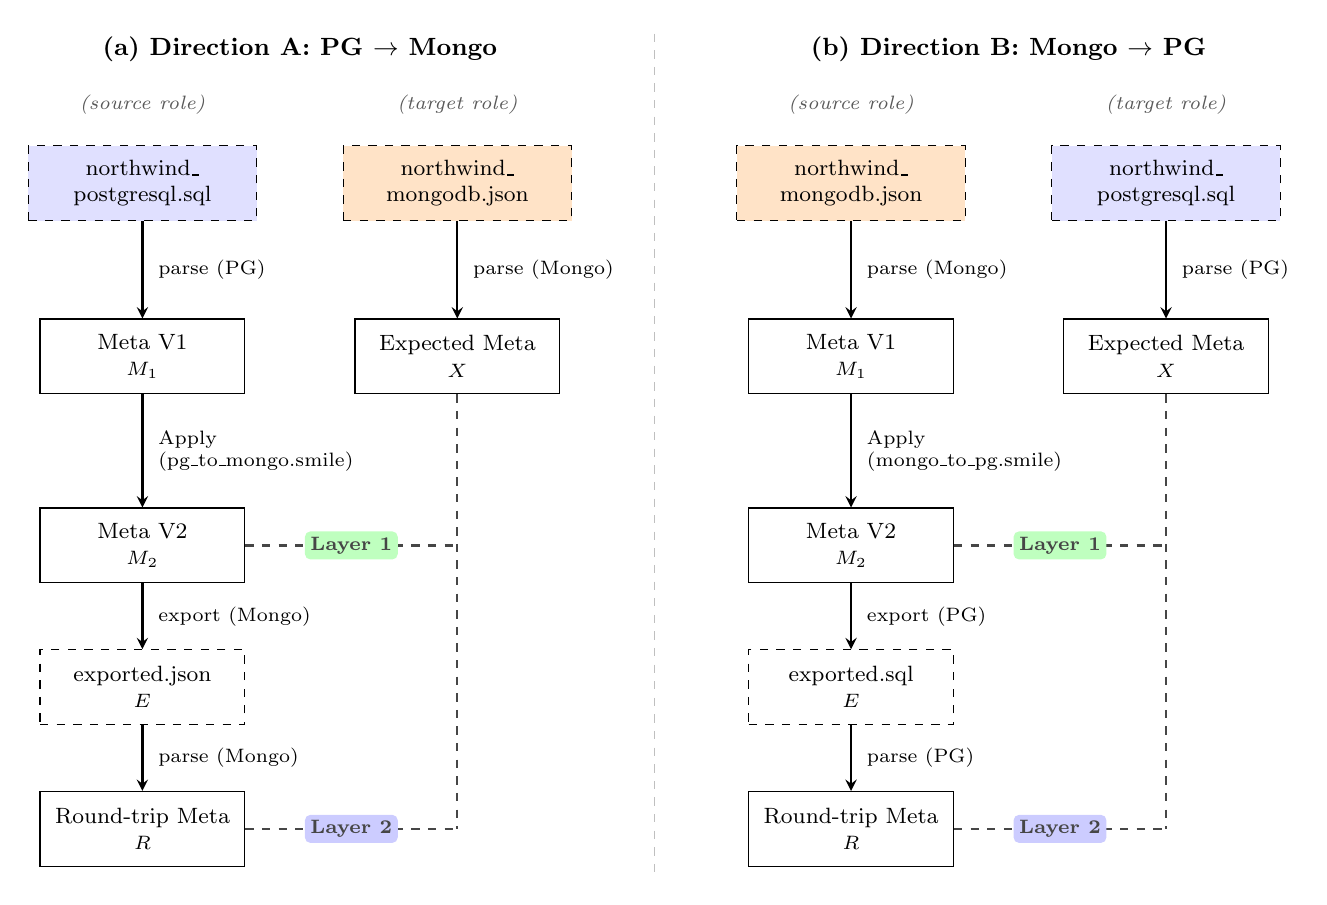
\begin{tikzpicture}[
    font=\footnotesize,
    data/.style={draw, rectangle, minimum height=0.95cm, minimum width=2.6cm,
                 align=center, inner sep=3pt},
    fileR/.style={draw, rectangle, dashed, minimum height=0.95cm,
                  minimum width=2.9cm, align=center, inner sep=3pt, fill=blue!12},
    fileD/.style={draw, rectangle, dashed, minimum height=0.95cm,
                  minimum width=2.9cm, align=center, inner sep=3pt, fill=orange!22},
    fileE/.style={draw, rectangle, dashed, minimum height=0.95cm,
                  minimum width=2.6cm, align=center, inner sep=3pt},
    arr/.style={->, >=stealth, thick},
    cmp/.style={dashed, thick, gray!55!black},
    rolelbl/.style={font=\scriptsize\itshape, text=gray!70!black},
  ]

  %% ================================================================
  %% Direction A (left panel): PG -> Mongo
  %% ================================================================
  \node[font=\small\bfseries] at (2.0, 1.7)
    {(a) Direction A: PG $\to$ Mongo};

  \node[rolelbl] at (0.0, 1.0)  {(source role)};
  \node[rolelbl] at (4.0, 1.0)  {(target role)};

  \node[fileR] (Asrc)  at (0.0,  0)    {northwind\_\\postgresql.sql};
  \node[fileD] (Atgt)  at (4.0,  0)    {northwind\_\\mongodb.json};

  \node[data]  (Av1)   at (0.0, -2.2)  {Meta V1\\\scriptsize $M_1$};
  \node[data]  (AX)    at (4.0, -2.2)  {Expected Meta\\\scriptsize $X$};

  \node[data]  (Av2)   at (0.0, -4.6)  {Meta V2\\\scriptsize $M_2$};
  \node[fileE] (Aexp)  at (0.0, -6.4)  {exported.json\\\scriptsize $E$};
  \node[data]  (Art)   at (0.0, -8.2)  {Round-trip Meta\\\scriptsize $R$};

  \draw[arr] (Asrc) -- node[right=2pt, font=\scriptsize]{parse (PG)}    (Av1);
  \draw[arr] (Atgt) -- node[right=2pt, font=\scriptsize]{parse (Mongo)} (AX);
  \draw[arr] (Av1)  --
    node[right=2pt, font=\scriptsize, align=left]{Apply\\(pg\_to\_mongo.smile)}
    (Av2);
  \draw[arr] (Av2)  -- node[right=2pt, font=\scriptsize]{export (Mongo)} (Aexp);
  \draw[arr] (Aexp) -- node[right=2pt, font=\scriptsize]{parse (Mongo)}  (Art);

  %% Vertical comparison rail (right column) and Layer connectors
  \draw[cmp] (AX.south) -- (4.0, -8.2);
  \draw[cmp] (Av2.east) --
    node[midway, fill=green!25, rounded corners=2pt, inner sep=2pt,
         font=\scriptsize\bfseries]{Layer 1}
    (4.0, -4.6);
  \draw[cmp] (Art.east) --
    node[midway, fill=blue!20, rounded corners=2pt, inner sep=2pt,
         font=\scriptsize\bfseries]{Layer 2}
    (4.0, -8.2);

  %% ================================================================
  %% Inter-panel divider
  %% ================================================================
  \draw[gray!50, dashed] (6.5, 1.9) -- (6.5, -8.8);

  %% ================================================================
  %% Direction B (right panel): Mongo -> PG
  %% ================================================================
  \node[font=\small\bfseries] at (11.0, 1.7)
    {(b) Direction B: Mongo $\to$ PG};

  \node[rolelbl] at (9.0,  1.0)  {(source role)};
  \node[rolelbl] at (13.0, 1.0)  {(target role)};

  \node[fileD] (Bsrc)  at (9.0,  0)    {northwind\_\\mongodb.json};
  \node[fileR] (Btgt)  at (13.0, 0)    {northwind\_\\postgresql.sql};

  \node[data]  (Bv1)   at (9.0,  -2.2)  {Meta V1\\\scriptsize $M_1$};
  \node[data]  (BX)    at (13.0, -2.2)  {Expected Meta\\\scriptsize $X$};

  \node[data]  (Bv2)   at (9.0, -4.6)  {Meta V2\\\scriptsize $M_2$};
  \node[fileE] (Bexp)  at (9.0, -6.4)  {exported.sql\\\scriptsize $E$};
  \node[data]  (Brt)   at (9.0, -8.2)  {Round-trip Meta\\\scriptsize $R$};

  \draw[arr] (Bsrc) -- node[right=2pt, font=\scriptsize]{parse (Mongo)} (Bv1);
  \draw[arr] (Btgt) -- node[right=2pt, font=\scriptsize]{parse (PG)}    (BX);
  \draw[arr] (Bv1)  --
    node[right=2pt, font=\scriptsize, align=left]{Apply\\(mongo\_to\_pg.smile)}
    (Bv2);
  \draw[arr] (Bv2)  -- node[right=2pt, font=\scriptsize]{export (PG)} (Bexp);
  \draw[arr] (Bexp) -- node[right=2pt, font=\scriptsize]{parse (PG)}  (Brt);

  \draw[cmp] (BX.south) -- (13.0, -8.2);
  \draw[cmp] (Bv2.east) --
    node[midway, fill=green!25, rounded corners=2pt, inner sep=2pt,
         font=\scriptsize\bfseries]{Layer 1}
    (13.0, -4.6);
  \draw[cmp] (Brt.east) --
    node[midway, fill=blue!20, rounded corners=2pt, inner sep=2pt,
         font=\scriptsize\bfseries]{Layer 2}
    (13.0, -8.2);

  \end{tikzpicture}%
  }%
  \caption{Two-layer validation pipeline for the forward (PG~$\to$~Mongo)
  and reverse (Mongo~$\to$~PG) direction.}
  \label{fig:dual-role-validation}
  \end{figure}

  Each panel of \autoref{fig:dual-role-validation} traces the full pipeline
  for a single direction. The left column propagates the source schema
  through reverse engineering to obtain Meta~V1, through the \textsc{Smile}
  transformation to Meta~V2, and through forward engineering followed
  by re-parsing to the round-trip meta. The right column reverse engineers
  the independently authored target file into the expected meta, against
  which Layer~1 compares Meta~V2 and Layer~2 compares the round-trip meta.
  Each box additionally carries the short symbol used in
  \autoref{alg:validation} ($M_1$, $M_2$, $X$, $E$, $R$) so that the
  diagram and the algorithm can be read in parallel. Reading the two
  panels together makes the dual role of the native files explicit:
  \texttt{northwind\_postgresql.sql} acts as the source in Direction~A
  and as the target in Direction~B, while \texttt{northwind\_mongodb.json}
  acts in the opposite roles. The fill colour of each file box is
  preserved across the panels to highlight this identity. The
  construction generalises across the four paradigm benchmark so that
  each of the four native schemas serves as source three times and as
  target three times, yielding the twelve cross paradigm directions
  without any manually constructed expected outputs.

  Layer~1 validates the correctness of the schema change expressed in
  \textsc{Smile}. It compares the transformed canonical schema (Meta~V2)
  with the expected target schema obtained by reverse engineering the
  corresponding ground truth target file. This layer therefore tests whether
  the script semantics produce the intended structural result independently
  of any target export. The methodology follows the compound operator
  validation pattern of Lerner~\cite{lerner2000model}, in which a sequence
  of schema modifications is evaluated by comparing the post evolution
  schema against an independently authored reference schema.

  Layer~2 validates the faithfulness of target export. It reverse engineers
  the schema generated by the target adapter and compares the resulting
  round trip meta representation with the same expected target schema.
  Conceptually, the adapter pair (forward engineering and reverse
  engineering) must satisfy the well behavedness condition of bidirectional
  transformations~\cite{foster2007combinators}, meaning an exported schema
  yields the same canonical meta representation when parsed again.

  Verdict synthesis is a derived label over the two layer outcomes, computed
  without any further comparison. The synthesis distinguishes four cases.
  \begin{itemize}
    \item \texttt{ok} when both layers pass.
    \item \texttt{smile\_script} when Layer~1 fails, indicating that the
          transformation produced the wrong Meta~V2.
    \item \texttt{adapter} when Layer~1 passes but Layer~2 fails, indicating
          that the export step diverged from the canonical Meta~V2.
    \item \texttt{unverifiable} when either layer is inapplicable, typically
          due to a missing ground truth target file.
  \end{itemize}
  This separation ensures that a failing test points unambiguously to a
  single responsible component rather than conflating script semantics and
  adapter implementation. \autoref{alg:validation} states the whole
  procedure compactly.

  \begin{algorithm}[htbp]
  \caption{Two layer validation with verdict synthesis.}
  \label{alg:validation}
  \begin{algorithmic}[1]
  \Require $M_2$ (migration result), $E$ (exported target), $T$ (target file), $\tau$ (target type)
  \Ensure verdict $\in \{\texttt{ok},\,\texttt{smile\_script},\,\texttt{adapter},\,\texttt{unverifiable}\}$
  \If{$T$ is not registered} \Return \texttt{unverifiable} \EndIf
  \State $X \gets \textsc{Adapter}_\tau.\textsc{parse}(T)$ \Comment{expected meta from ground truth}
  \If{$\tau = \textsf{Document}$} \State $M_2 \gets \textsc{path\_normalize}(M_2)$ \EndIf
  \State $L_1 \gets (M_2 = X)$ \Comment{Layer 1: \textsc{Smile} script correctness}
  \State $R \gets \textsc{Adapter}_\tau.\textsc{parse}(E)$
  \State $L_2 \gets (R = X)$ \Comment{Layer 2: adapter forward engineering correctness}
  \If{$L_1 \land L_2$} \Return \texttt{ok} \EndIf
  \If{$\lnot L_1$} \Return \texttt{smile\_script} \EndIf
  \State \Return \texttt{adapter}
  \end{algorithmic}
  \end{algorithm}

  \paragraph{Design rationale.}
  A natural alternative to the parse-then-compare construction
  underlying Layer~2 would be a direct comparison between the exported
  native file $E$ and the target native file $T$. The construction is
  preferred because, for schema-flexible paradigms, no useful notion
  of equivalence is available at the native-text level. The same
  logical schema admits structurally distinct but equally valid native
  representations: a MongoDB schema may be expressed with embedded
  sub-documents or with cross-collection references, and with a single
  root document or with a top-level \texttt{collections} envelope; a
  Neo4j schema may attach a given attribute to a node or to a
  relationship; a Cassandra schema may denormalise the same logical
  record under several partition and clustering key choices. Whether
  two such representations should count as equivalent depends on a
  paradigm-specific canonical interpretation, and that interpretation
  is precisely what each adapter's reverse-engineering parser already
  encodes. Reimplementing that interpretation at the diff level would
  duplicate parser logic without adding coverage; reusing the existing
  parsers as canonicalisers and lifting the comparison to the
  meta-model level instead yields an unambiguous notion of structural
  equivalence defined by \textsc{compute\_diff} on the canonical
  \textsc{Database} object. Under the assumption that Layer~1 holds
  ($M_2 = X$), Layer~2 then reduces to
  $\textsc{parse}(\textsc{export}(X)) = X$, which is precisely the
  PUT-GET law of well-behaved bidirectional
  transformations~\cite{foster2007combinators}; this framing isolates
  adapter self-consistency as a property tested independently of the
  script and preserves the unambiguous attribution of failures to
  either the script or the adapter.

  \section{Coverage Results}\label{sec:eval-coverage}

  All 32 Northwind configurations pass both validation layers. What is
  left in the report is 7 nullability notices of the form                                                                                                                 ``\texttt{is\_optional} differs between actual and expected'', and
  every one of them traces back to a residual \texttt{NOT NULL} flag
  inherited from a structural element of the source schema rather
  than to a missing structural change.

  \begin{table}[htbp]
  \centering
  \caption{Validation results across 32 Northwind test scripts.}
  \label{tab:eval-results}
  \renewcommand{\arraystretch}{1.15}
  \begin{tabular}{l c c c c}
  \toprule
  \textbf{Category} & \textbf{Configs} & \textbf{Layer 1} & \textbf{Layer 2} & \textbf{Notices} \\
  \midrule
  Same-model          & 8  & 8/8   & 8/8   & 2  \\
  Cross-model         & 24 & 24/24 & 24/24 & 5 \\
  \midrule
  \textbf{Total}      & \textbf{32} & \textbf{32/32} & \textbf{32/32} & \textbf{7} \\
  \bottomrule
  \end{tabular}
  \end{table}

  In the Notices column each (direction, field) pair is counted once.
  The two grammar variants of a direction count as one entry. The
  specific and the generalised grammar produce identical Meta V2
  output and raise the same notice.

  All 7 notices share a single signature. The SMILE result reports
  \texttt{is\_optional=False} while the ground truth has
  \texttt{is\_optional=True}. Most of them come from Cassandra,
  since its partition and clustering keys are inherently
  \texttt{NOT NULL} at the storage layer, and that flag stays on the
  column even after the key itself has been removed. The mismatch
  shows up across six distinct directions.
  \begin{itemize}
    \item C2D, C2G, and C2R for \texttt{orders.order\_date}, a
          clustering key in V1 that the relational, document, and
          graph targets all leave nullable.
    \item C2C for \texttt{products.supplier\_id}, part of the V1
          partition key and demoted to a regular nullable column
          in V2.
    \item R2C for \texttt{orders.employee\_id} and
          \texttt{orders.shipper\_id}, \texttt{NOT NULL} FK columns in
          PostgreSQL that SMILE carries forward, while the Cassandra
          V2 ground truth leaves them nullable.
    \item G2G for \texttt{contact.customer\_id}, a NODE KEY in V1
          customers brought along by SPLIT into the new contact node,
          where the V2 design treats it as a regular nullable
          property.
  \end{itemize}
  Grouped by the structural origin of the residual \texttt{NOT NULL}
  flag rather than by direction, the same 7 notices reduce to three
  paradigm-bound categories. Four come from Cassandra storage-layer
  keys, with three clustering-key occurrences in C2D, C2G, and C2R
  plus one partition-key occurrence in C2C. Two come from explicit
  PostgreSQL \texttt{NOT NULL} FK declarations propagated to a
  Cassandra target in R2C. The remaining one comes from a Neo4j
  NODE KEY carried into a new node through SPLIT in G2G.

  None of these notices invalidate the structural result or change
  the verdict. They are the canonical meta model doing what it should.
  The model surfaces paradigm level nullability differences instead
  of absorbing them silently.

  The implementation deliberately leaves these gaps visible. Silencing
  them inside the adapters would yield validation reports with zero
  notices, but it would also erase the very semantic distinction that
  motivates a typed canonical meta model. M-Model+ is meant to
  abstract paradigm neutral structure such as entities, properties,
  and constraints, without conflating paradigm specific semantics like
  \texttt{is\_optional}. The 7 notices are therefore intentional
  artefacts. Each records a single property whose \texttt{NOT NULL}
  flag came from a structural element of the source paradigm. The
  source element might be a Cassandra partition or clustering key, a
  PostgreSQL \texttt{NOT NULL} FK column, or a graph node key carried
  through SPLIT. The target paradigm leaves the same column nullable
  by default.
  Automatic normalisation would swap this visibility for silent
  rewrites, and the meta model would lose its claim to being a
  faithful canonical representation. The notice surface is therefore a
  feature of the validation report, not a defect to be eliminated.
  \section{Summary}\label{sec:eval-summary}

